%%
%% EXPERIMENTS AND RESULTS
%%
\chapter{Mixture Models and 0-1 data}
\label{ch:mixturemodels}
\begin{fquote}[Samuel Karlin]The purpose of models is not to fit the data but to sharpen the questions.\fqsource{$11^{th}$ R A Fisher Memorial Lecture (1983)} \end{fquote} 

\begin{synopsis}
This chapter is devoted to the introduction of the mathematical foundation of mixture models, special consideration is on the finite mixture models of multivariate Bernoulli\footnote{Bernoulli Distribution is named after Swiss scientist Jacob Bernoulli(1654-1705)} distributions. The chapter also covers EM algorithm~\cite{wolfe, expectmax} and its formulation for the finite mixture models of multivariate Bernoulli distributions~\cite{wolfe, everittmixdist}. The chapter also provides brief introduction to cross-validation, a method for accessing the results of statistical analysis. Near the end of the chapter, it shortly reviews the literature on the use of finite mixture models of multivariate Bernoulli distributions with a focus on cancer genetics. Part of work discussed in this chapter has been published in~\cite{premup}~and~\cite{premprib}.
\end{synopsis}

\section{0-1 Data}
\label{s:binarydata}
History of collection of information and data is quite long. However, the size of data and information was relatively small. Recently improved technology, increased storage capacity, and more importantly the realization of importance of data has lead to the collection and storage of data. Moreover, as discussed in Chapter~\ref{ch:introduction}, recent technologies are producing data at exponential rates. Thus, extracting meaningful information from those data is a matter of extreme urgency. In all the fields of study ranging from biology through astronomy to social sciences, 0-1 data has been of special interest. 0-1 data is a special class of categorical data with only two scales which can be considered as true or false, success or failure. In other words, 0-1 data captures the dichotomy of two classes. 0-1 data have only two classes (categories) and often represented as \textbf{0} and  \textbf{1} or \textbf{1} and \textbf{-1}. 0-1 data naturally occur in many areas of study: in social science, interview questions relating to marital status, gender, like or dislike, alive or dead can be formulated as 0-1 data. Similarly, in palaeontology 0 can represent absence of fossils and 1 can represent presence of fossils~\cite{Puolamaki06pcbi}. In universities, the relationship between courses and the students can be represented as 0-1 data where 1 represents that the student has taken the course and 0 represents that the student has not taken the course as discussed and preprocessed in~\cite{randomization}. One of the principal uses of the 0-1 data is in \textbf{`Market Basket Data'} which assembles information about whether a customer has bought certain goods or not. One of the popular benchmark dataset RETAIL is a prominent example of a market basket data~\cite{retail}. Over the years biology and genetics, have been one of the major sources of 0-1 data. For example, 0-1 data can capture the notion of presence or absence of certain characteristics in species. 0-1 data analyzed in this thesis as discussed in Section~\ref{s:dataset} is also a 0-1 data denoting the presence or absence of chromosomal aberrations in chromosome bands. 


\section{Mixture Models}
\label{s:mixmodels}
Probabilistic modeling aims to approximate the probability of an event occurring again on the basis of limited instances of observed data. The estimated probability distribution aims to explain the process of data generation. FMM (Finite Mixture Models) are probabilistic models with varying uses such as density estimation, clustering, classification~\cite{bishop, everittmixdist, mclachlanfmm}. These models belong to an interesting and flexible model family for modelling latent (unobserved) variables in complex distributions. Finite Mixture Models have a very long history. Geoffrey McLachlan and David Peel in their book \textit{``Finite Mixture Models''} attribute famous biometrician Karl Pearson for the first use of the mixture models where he fitted two Gaussians with different means ($\mu _1$ and $\mu _2$) and variances ($\sigma _1 ^ 2$ and $\sigma _2 ^ 2$) in proportions $\pi _1 $ and $\pi _2$ for some data in 1894~\cite{mclachlanfmm}. However, the popularity of mixture models has significantly grown over the past few decades because of the dramatic increase in computing power. Nonetheless,  the major share of contribution goes to the mathematical foundation, formulation and understanding of the mixture models. Furthermore, formulation of the EM algorithm~\cite{expectmax}, which provides a conceptual framework to estimate the maximum likelihood from the incomplete data, in 1977 provided the necessary impetus to the growing use of mixture models. Over the few years, finite mixture models have been extensively used in many application domains including model based clustering, classification, image analysis, and collaborative filtering in analysis of high dimensional data. 

\begin{figure}[h!]
\centering
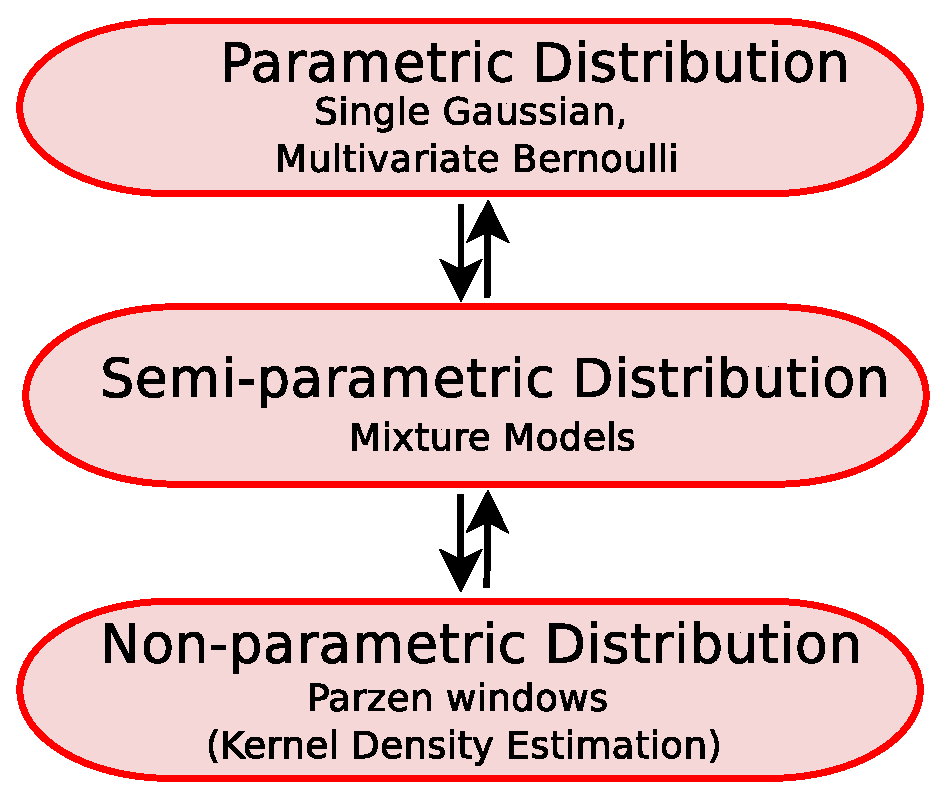
\includegraphics[width=0.5\textwidth]{figures/semipara}
\caption[Different types of distributions]{Schematic representation of different forms of distributions.}\label{Fig:semiparametric}
\end{figure}


FMM (Finite Mixture Models) models a statistical distribution by a mixture (or weighted sum) of simple distributions such as Gaussian, Poisson and Bernoulli. It decomposes the density function into a set of component density functions. Each of the decomposed density functions defines a specific class of the origination of the data i.e each component density functions represents a portion of original distribution. This form of representation is not possible with other simple parametric distributions. The basic assumption of FMM is that the different classes\footnote{The class here is not similar to the class labels.} in the data originate from the well-known parametric distributions. Except for this assumption of the data source, FMMs are extremely flexible in the choice of the distribution. Any classical parametric distributions such as Normal(Gaussian), Poisson~\cite{poission}, Bernoulli can be chosen as component density function. Unlike the case with one Bernoulli, determining the training sample contributing to a particular component is not possible. Hence, the methods based on mean and covariance matrix are not applicable to the mixture models. 

After the choice of distribution, the primary task is then to estimate the parameters of the selected distribution such as mean ($\mu$) and variance ($\sigma ^2 $) for Gaussian distribution; rate of occurrence ($\lambda $) for Poisson distribution~\cite{poission}. It is important to note that each component distribution will be defined by its own set of parameters thus differing itself from the others. This explains the reason why mixture models are called semi-parametric models as depicted in the Figure~\ref{Fig:semiparametric}. The complexity of mixture models depends on the complexity of the problem being solved, not the size of dataset.  In this thesis, 0-1 data is analyzed and the assumption is that it follows the Bernoulli distribution. Bernoulli distribution of a single random variable is parameterized by one parameter $\theta$ which denotes the probability of success in a trial with two possible outcomes: success and failure. The learning task is then limited to learning the Bernoulli parameter~$\theta$.

%If the number of mixture components in the mixture model is fixed based on some prior knowledge, then the mixture model acts as a parametric model. On the other hand, if the number of mixture components is not fixed initially but is allowed to learn from the data then the mixture model can be considered a non-parametric model.




\subsection*{Advantages of Mixture Models}
\label{ss:whymixmodels}
Mixture Models have various merits and are often a suitable choice for modelling data. Some of the most useful characteristics of mixture models can be summarized as the following:
\begin{itemize}
 \item A mixture model learns the structure in the data better than most other methods as the different component distributions capture the dominant patterns present in the data. 
 \item Learning mixture models involve well studied statistical inference techniques~\cite{mclachlanfmm}. 
 \item Mixture models are flexible in terms of the choice of the component distributions.
 \item Mixture Models can generate leptokurtic distributions from mesokurtic ones~\cite{pdeb}.
 \item Mixture Models can also generate skewed distributions from symmetric components~\cite{pdeb}.
 \item It is suitable for any form of data either discrete or continuous.
 \item When mixture models are used in clustering, the components represent the clusters thus making it possible to obtain density estimation for each cluster.
 \item Mixture models also provides the facilities for soft classification~\cite{pdeb}. 
\end{itemize}

Mixture models are flexible models and have varying uses. Some of the basic areas where mixture models are most prevalent are:
\begin{itemize}
 \item \textbf{Clustering:} Mixture models are at the heart of model based clustering where each component denotes one cluster.
 \item \textbf{Handling Missing Data:} Mixture models have also been extensively used to handle the missing data for building the model~\cite{mclachlanfmm}.
 \item \textbf{Density Estimation:} In Bayesian statistics, mixture models can be used to assign the flexible priors~\cite{mclachlanfmm}.
 \item \textbf{Model Averaging:} Mixture models have often been used to combine different density models~\cite{bishop}.
 \item \textbf{Modelling Heterogeneity:} Here in this thesis mixture models have been used to model the heterogeneous cancer cases in different patients.  
\end{itemize}

\subsection*{Mixture of Multivariate Bernoulli Distributions}
\label{ss:mixmulber}
The major focus of the thesis is concentrated on modelling DNA copy number aberrations which is 0-1 data. Hence, the mixture of multivariate Bernoulli distributions forms the crux of the thesis. 

Univariate Bernoulli distribution is a probability distribution with two possible outcomes: success and failure~\cite{probability}. Consider an example of a single random binary variable, $x \in \{ 0,1\}$ where $x=0$ denotes the failure of an event and $x=1$ denotes the success of an event or other similar dichotomy such as success or failure of an event and the coin tossing. For example, success of an event may be a student participating a course and failure of an event may be the student not participating in the course~\cite{randomization}. Let the probability of occurrence of $x=1$ be $\theta$ such that $0 \le \theta \le 1$. Therefore, the probability of occurrence of $x=0$ is $1-\theta$. Thus, $p(x=1|\theta)=\theta$ and $p(x=0|\theta)=1-\theta$. Accordingly, the probability mass function i.e. probability distribution~\cite{probability, bishop} over $x$ is given by the equation 
\begin{eqnarray}
p(x|\theta)=\theta ^ {x }(1-\theta)^{1-x}
\end{eqnarray} 
The mean or the expected value of the random binary variable is given by 
\begin{eqnarray}
\mathbb{E}[x] = 0 \times p(x=0|\theta)+1 \times p(x=1|\theta) =  p(x=1|\theta) = \theta
\end{eqnarray} 
The variance of the random binary variable is defined as the dispersion of random variable. It can be obtained by
\begin{eqnarray}
var(x)= \mathbb{E}(x^{2}) - \{ \mathbb{E}(x)\}^{2} 
\end{eqnarray}
where 
\begin{eqnarray}
\mathbb{E}(x^{2})= 0^{2} \times p(x=0|\theta) + 1^{2} \times p(x=1|\theta)=p(x=1|\theta)=\theta  \nonumber
\end{eqnarray}
and also
\begin{eqnarray}
\{ \mathbb{E}(x)\}^{2} = \theta^{2}  \nonumber
\end{eqnarray}
Therefore, 
\begin{eqnarray}
var(x)=\theta - \theta ^{2} = \theta (1-\theta)
\end{eqnarray}

The probability $p(x|\theta)$ can be extended to the binary space $\{0,1\}^{N}$ i.e. to a dataset $\underline{\overline{X}}= \{ \overline{X}_1 ,\ldots , \overline{X}_d \}$ and $\overline{X}_1 = \left( X_{11}, X_{12} \ldots X_{1d}\right)$~\cite{bishop}. Here,  $\left( X_{11}, X_{12} \ldots X_{1d}\right)$ are the observed values of $\underline{\overline{{X}}}$. Hence, the probability mass function of the multivariate Bernoulli distribution is given by

\begin{eqnarray}
\label{eq:1}
P(\mathcal{D}|\Theta)=\displaystyle\prod_{i=1}^{\mathrm{d}}p(x_i|\theta) = \displaystyle\prod_{i=1}^{\mathrm{d}} \theta_i ^{x_i}(1-\theta _i)^{1-x_i}
\end{eqnarray} 

where $\theta \in \mathbb{R}^i$ and $0 \leq \theta _i \leq 1$ for all $1 \leq i \leq \mathrm{d}$ and $x_1, x_2, \ldots x_\mathrm{d} = \mathbf{x} \in \{0,1\}^\mathrm{N}$

\begin{figure}[h!]
\centering
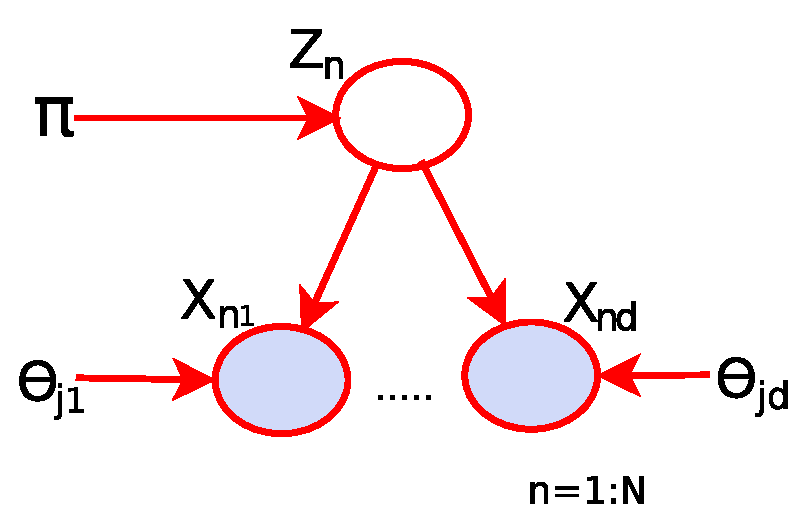
\includegraphics[width=0.5\textwidth]{figures/bmm}
\caption{A graphical mixture model of mixture of Bernoulli.}\label{Fig:bmm}
\end{figure}

This can be represented as the DGM (Directed Graphical Model), which is a type of DAG (Directed Acyclic Graph)~\cite{bishop} as shown in Figure~\ref{Fig:bmm} which is similar to Naive Bayes classifier except that the class labels $Z_n$ is hidden.

The likelihood function in Equation~(\ref{eq:1}) is a function of $\theta$. For independent and identically distributed samples $\overline{{X}}=\{x_n\} ^{\mathrm{N}}_{n=1}$ from $\{ 0, 1\}^{\mathrm{N}}$, the vector $\hat{\theta}$ that maximizes the likelihood function in Equation~(\ref{eq:1}) is the estimated value of $\theta$. The joint probability for the $N$ samples of data is given by:

\begin{eqnarray}
\label{eq:0}
\mathrm{ln} \; (P(X_1, X_2 \ldots X_N)) & = & \mathrm{ln} \; \displaystyle\prod_{i=1}^{\mathrm{N}} p(x_i) \nonumber \\
\mathrm{ln} \;\displaystyle\prod_{i=1}^{\mathrm{N}} p(x_i) & = & \displaystyle\sum_{i=1}^{\mathrm{N}} \mathrm{ln} p(x_i) 
\end{eqnarray}

Furthermore, maximizing the likelihood function in Equation~(\ref{eq:1}) equivalent to maximizing the logarithm of the likelihood. Thus,

\begin{eqnarray}
\label{eq:2}
\mathrm{ln} \; p(\mathcal{D}|\Theta)=\displaystyle\sum_{i=1}^{\mathrm{d}} ln \; p(x_i|\theta_i) = \displaystyle \sum _{i=1} ^{\mathrm{d}} x_i \; ln \; \theta_i +(1-{x_i})(1-\theta_i)
\end{eqnarray} 

From Equation~(\ref{eq:2}) it can be seen that the log likelihood function depends on the $\mathrm{d}$ samples of $x_d$ through the sum $\displaystyle\sum_{i=1}^{\mathrm{d}} x_n$ which provides adequate statistics about the distribution. Taking the derivative of (\ref{eq:2}) with respect to $\theta$ and equating it to zero gives the value of maximum likelihood estimation. The value is given by:

\begin{eqnarray}
\label{eq:3}
\hat{\theta}_{\mathrm{ML}} = \frac{1}{N} \displaystyle\sum_{i=1}^{\mathrm{N}}x_i
\end{eqnarray} 

The Definition~(\ref{eq:3}) is also known as the sample mean. If the sample $\overline{{X}}$ contains higher order correlations, the sample covariance matrix will be diagonal. Hence, the maximum likelihood estimator in Equation~(\ref{eq:3}) gives unsatisfiable result. 

Assuming that the data comes from a mixture of known number of the components, $J$, finite mixture of multivariate Bernoulli distributions is defined as:

\begin{eqnarray}
\label{eq:maindist}
 p(\mathcal{D}|\Theta)=\displaystyle\sum_{j=1}^{\mathrm{J}} \pi_j P_j(x|\theta_j)
\end{eqnarray}

In Definition~(\ref{eq:maindist}) each $P_j$ is a multivariate Bernoulli Distribution parameterized by $\theta_j$. Hence, the finite mixture model for multivariate Bernoulli distribution can be formulated as:

\begin{eqnarray}
\label{eq:4}
 p(\mathcal{D}|\Theta)=\displaystyle\sum_{j=1}^{\mathrm{J}} \pi_j \displaystyle \prod _{i=1} ^{\mathrm{d}} \theta_{ji}^{x_i} (1-\theta_{ji})^{1-x_i}
\end{eqnarray} 

where $\pi_j$ are the mixture proportions satisfying the properties such as convex combination such that $\pi_j \geq 0 $ and $\displaystyle\sum_{j=1}^{\mathrm{J}} \pi_j = 1$ for all $j=1, \ldots J$. The model parameters, $\Theta$, is composed of $\theta_1, \theta_2, \theta_3 \ldots \theta_d$ for each component distribution. The combination of $J$ mixtures of multivariate distribution in Equation~(\ref{eq:4}) can capture the correlations (the clustering structure) in the sample $\overline{{X}}$ thus solving the problem of unsatisfiable result in Equation~(\ref{eq:3}). Finite mixture of multivariate Bernoulli distributions with  number of components equals to $J$ and dimension of dataset $=d$ is parametrized by $\Theta=\{J$, $\{ \pi_j, \theta_j\}_{j=1}^{J}\}$ for each component distribution.

Fitting the Bernoulli Mixture Model involves learning the parameters $\Theta$ and the number of components $J$ from the given data sample $\overline{{X}}$. This can be formulated in terms of loglikelihood as:

\begin{eqnarray}
\label{eq:loglkhood}
\mathcal{L} (\Theta)= \displaystyle\sum_{n=1}^{\mathrm{N}} log \; P(x_n|\Theta) = \displaystyle\sum_{n=1}^{\mathrm{N}} log  \left [ \displaystyle\sum_{j=1}^{\mathrm{J}} \pi_j \displaystyle \prod _{i=1} ^{\mathrm{d}} \theta_{ji}^{x_{ni}} (1-\theta_{ji})^{1-x_{ni}} \right]
\end{eqnarray} 

%\begin{eqnarray}
%\label{eq:lkhood}
%\mathcal{L} = \displaystyle\sum_{n=1}^{\mathrm{N}} log  \left [ \displaystyle\sum_{j=1}^{\mathrm{J}} \pi_j \displaystyle \prod _{i=1} ^{\mathrm{d}} \theta_{ji}^{x_i} (1-\theta_{ji})^{1-x_i} \right]
%\end{eqnarray} 

The Equation~(\ref{eq:loglkhood}) can be maximized with high number of mixture components i.e. the mixture models gets high likelihood values for the training set. However, large number of mixture components increases model complexity and often results in overfitted model generalizing poorly on future data. On the other hand, smaller number of mixture components results in underfitting. To find the trade-off between the appropriate model complexity and large value of the Equation ~(\ref{eq:loglkhood}) some validation techniques must be used. The basic aim of the thesis is to achieve maximally simple and compact parsimonious models. Parsimonious models are the models having as few parameters as possible for a given quality of a model. There are different principles for developing parsimonious models such as Ockham's razor~\cite{occam}. In this thesis, $10$-fold cross-validation discussed in Section~\ref{s:crossvalidation} is used for the same purpose. The maximization of the Equation~(\ref{eq:loglkhood}) can be performed by using EM algorithm discussed in Section~\ref{s:em}.

One of the major drawbacks of finite mixture models of multivariate Bernoulli distributions is that it belongs to the class of non-identifiable distributions~\cite{nonidentifiable}. Thus, there exists distinct parameters ($\alpha$ , $\theta$) and ($\beta$ , $\lambda$) such that they represent same distribution excluding the trivial permutations. The problem of non-identifiability has been extensively studied in literature after it was proved in~\cite{nonidentifiable, furthernoni} that these FMMs are non-identifiable. However, studies in~\cite{furthernoni} have proved that in spite of their non-identifiable nature, they are useful in various applications. 

\subsection*{Challenges in Using Mixture Models}
\label{ss:challanges}
In spite of great virtues of mixture models, there are several major challenges in the estimation of mixture models. The mixture models require that the number of components be known \textit{apriori}. Even if the models are known \textit{apriori}, it is often difficult to reliably distinguish different components. In worst case scenario, some of the components may simply converge to the outliers present in the data. It is important to note that selection of the number of mixture components directly influences the performance of the mixture models. Lesser the number of components, the mixture model behaves similar to a simple parametric model and increases the bias. On the contrary, if the mixture model has a large number of components, the model can overfit the data thus producing unreasonable variation. Hence, there is always a trade-off between the two. Secondly, the likelihood function may have multiple local maxima. In order to address these challenges we use $10$-fold cross-validation repeated 50 times so that we get the optimal results. Thirdly, the major drawback in using mixture models is the computational complexity of training the mixture models. Normally, training mixture models is computationally expensive when compared with other parametric (such as Poisson distribution~\cite{poission}) as well as non-parametric (such as k-means~\cite{kmeans, kmeans2}) methods. 


\section{Expectation Maximization Algorithm}
\label{s:em}
Different methods have been proposed and implemented to estimate the parameters of the mixture model including EM (Expectation Maximization)~\cite{wolfe, expectmax}, MCMC (Markov Chain Monte Carlo)~\cite{mcmcintro}, and Spectral Method~\cite{spectralmethod1, spectralmethod}. MCMC uses Gibbs sampling to sample from posterior distribution. Spectral method, on the other hand, uses SVD (Singular Value Decomposition)~\cite{matrixcomputation, svdgolub} on the data. For distributions satisfying specific separation condition, spectral method estimates the mixtures highly similar to the true mixture with high probability~\cite{spectralmethod}. However, in this thesis EM algorithm, is used to estimate the parameters of the mixture model in a cross-validation setting to justify the selection of the number of component distributions.

Given a sample $\overline{{X}}$, the parameters maximizing $\Theta$ and $J$ can not be ascertained analytically. However, EM algorithm can be used to optimize the parameters. The Expectation Maximization (EM) is an iterative algorithm for the computation of maximum likelihood with broad application areas and was first coined by Dempster, Laird and Rubin in~\cite{expectmax}. The EM algorithm gets its name because in each iteration of EM algorithm comprises two steps: Expectation Step (E-Step) and Maximization Step (M-Step).

Componentwise differentiation of the Term~(\ref{eq:loglkhood}) with respect to $\theta$ and $\pi$ results in:
\begin{eqnarray}
\label{eq:em1}
\frac{\delta \mathcal{L}}{\delta \pi_{j}} = \frac{1}{\pi_{j}} \displaystyle\sum_{n=1}^{\mathrm{N}} P(j|x_n;\pi,\Theta)-N \quad j=1, \ldots, J
\end{eqnarray} 
And also
\begin{eqnarray}
\label{eq:em2}
\frac{\delta \mathcal{L}}{\delta \theta_{ji}} = \frac{1}{\theta_{ji}(1-\theta_{ji})} \displaystyle\sum_{n=1}^{\mathrm{N}}P(j|x_n;\pi,\Theta) (x_{ni}-\theta_{ji}) \\
where \quad j=1, \ldots, J \; and \; i=1,\ldots, d \nonumber
\end{eqnarray} 

The term -N in equation satisfies the constraint $\sum_{j=1}^{J}\pi_j$ introduced in loglikelihood via Lagrange multiplier. Now, From Bayes' theorem the posterior probability can be calculated as shown below.
\begin{eqnarray}
\label{eq:em3}
P(j|x_n;\pi,\Theta) & = & \frac{p(x_n|j;\pi,\Theta)p(j)}{\sum_{j'=1}^{J} P(x_n|j';\pi\Theta)p(j')} \nonumber \\
& = & \frac{\pi_j \prod_{i=1}^{d} \theta_{ji}^{x_{ni}}(1-\theta_{ji})^{1-x_{ni}}} {\sum_{j'=1}^{J} \prod_{i=1}^{d} \theta_{j'i}^{x_{ni}}(1-\theta_{j'i})^{1-x_{ni}}} 
\end{eqnarray}

Derivation of the EM algorithm is fairly simple and can be referred from the works of Everitt and Hand~\cite{everittmixdist} as well as Wolfe~\cite{wolfe}. The basic equations of EM algorithm are:

\textbf{E-step:} E-step computes the posterior probability using the Equation~\ref{eq:em3} for the most recent values of parameters {$\theta ^{\tau}, \Theta ^{\tau}$} at iteration $\tau$ i.e. calculate $P(j|x_n;\pi ^{\tau},\Theta ^{\tau})$

\textbf{M-step:} M-step recomputes the the values of parameters {$\theta ^{\tau+1}, \Theta ^{\tau+1}$} for the next iteration.

\begin{eqnarray}
\label{eq:mstep1}
\pi_{j}^{\tau+1} & = & \frac{1}{N} \displaystyle \sum _{n=1}^N P(j|x_n;(\pi^{(\tau)}),\Theta^{(\tau)}) \nonumber \\
\Theta_{j}^{(\tau+1)} & = & \frac{1}{N \pi_{j}^{(\tau+1)}} \displaystyle \sum _{n=1}^N P(j|x_n;(\pi^{(\tau)}),\Theta^{(\tau)})x_n 
\end{eqnarray}

Iterations between E and M step produce a succession of monotonically increasing sequence of values of loglikelihood for the parameters $\tau\;=\;0,1,2,3\ldots$ regardless of the starting point $\{\pi^{(0)},\Theta^{(0)}\}$. This result is advantageous but also results in the problem of singularities, the possibility of getting an infinite likelihood if a single data point is assigned to one of the mixtures. However, mixture of Bernoulli distribution are not susceptible to the problem of singularities because the likelihood function is bounded by the constraint $0\leq p(x_n|\theta_j) \leq 1$ except for some trivial cases such as: assume that data is 1 but model is 0, so the likelihood of the model is 0 and if we take the loglikelihood it turns out to be $\mathrm{log} 0 = \infty $. Furthermore, loglikelihood surface is unbounded. Such problems, however, are rare in multivariate case. EM requires that the number of the mixture components in the mixture model be known in advance. Furthermore, EM algorithm is sensitive to the initializations and the results may differ on the same data for different initializations. Nevertheless, EM algorithm is deterministic with given initializations and a given dataset. EM algorithm can get stuck in local minima and the global optimal results are not often guaranteed. To overcome these problems regularization techniques as discussed in~\cite{regularization} can be used. In spite of these demerits, EM algorithm has been widely used because of its reliability.

One of the important issues to note regarding the non-identifiable problem is that it matters least with respect to this thesis. Our main aim is to maximize the Equation~(\ref{eq:loglkhood}) considering the trade-off between the model complexity (number of components in the mixture model) and small difference in the maximum likelihood value. If different parameters satisfy the trade-off, choosing any of those parameters will have negligible effect on the final results. 

\section{Cross-validation}
\label{s:crossvalidation}

The idea of cross-validation, sometimes also called rotation estimation and pioneered by \cite{crossvalind} and \cite{monsteller}, is fundamental concept in machine learning for assessing the results of the statistical analysis. Various forms of cross-validation techniques have been proposed. The basic definition of $k$-fold cross-validation
states that the training set $\mathcal{T}$ is divided into $k$ exhaustive and exclusive equal sized sub-sets $\mathcal{T}_1$, $\mathcal{T}_2$, $\ldots \mathcal{T}_k$. The main assumption is that the both the training and the validation sets are independent. For each sub-set $\mathcal{T}_i$ where $i \in 1, 2, 3 \ldots k$ the data is trained on the union of all the other subsets and determine the error on the subset $\mathcal{T}_i$. The final error of the algorithm is the average error on all the sub-sets as shown in the Equation~\ref{eq:errorcv}.

\begin{eqnarray}
\label{eq:errorcv}
\varepsilon =\frac{1}{k} \sum_{i=1}^{k} \epsilon_{i}
\end{eqnarray}


The initial subset of data is called the test set; while union of the remaining subsets is called the training set. The efficiency of $k$-fold cross-validation largely depends on the choice of $k$. If the number of $k$ is small, the algorithm is computationally efficient as it requires performing lesser rounds of experiments. Furthermore, the variance of the estimator will be negligible. On the contrary, the bias of the estimator will be significantly larger, larger than the true error (generalization error) on the future data. 

\begin{figure}[h!]
\centering
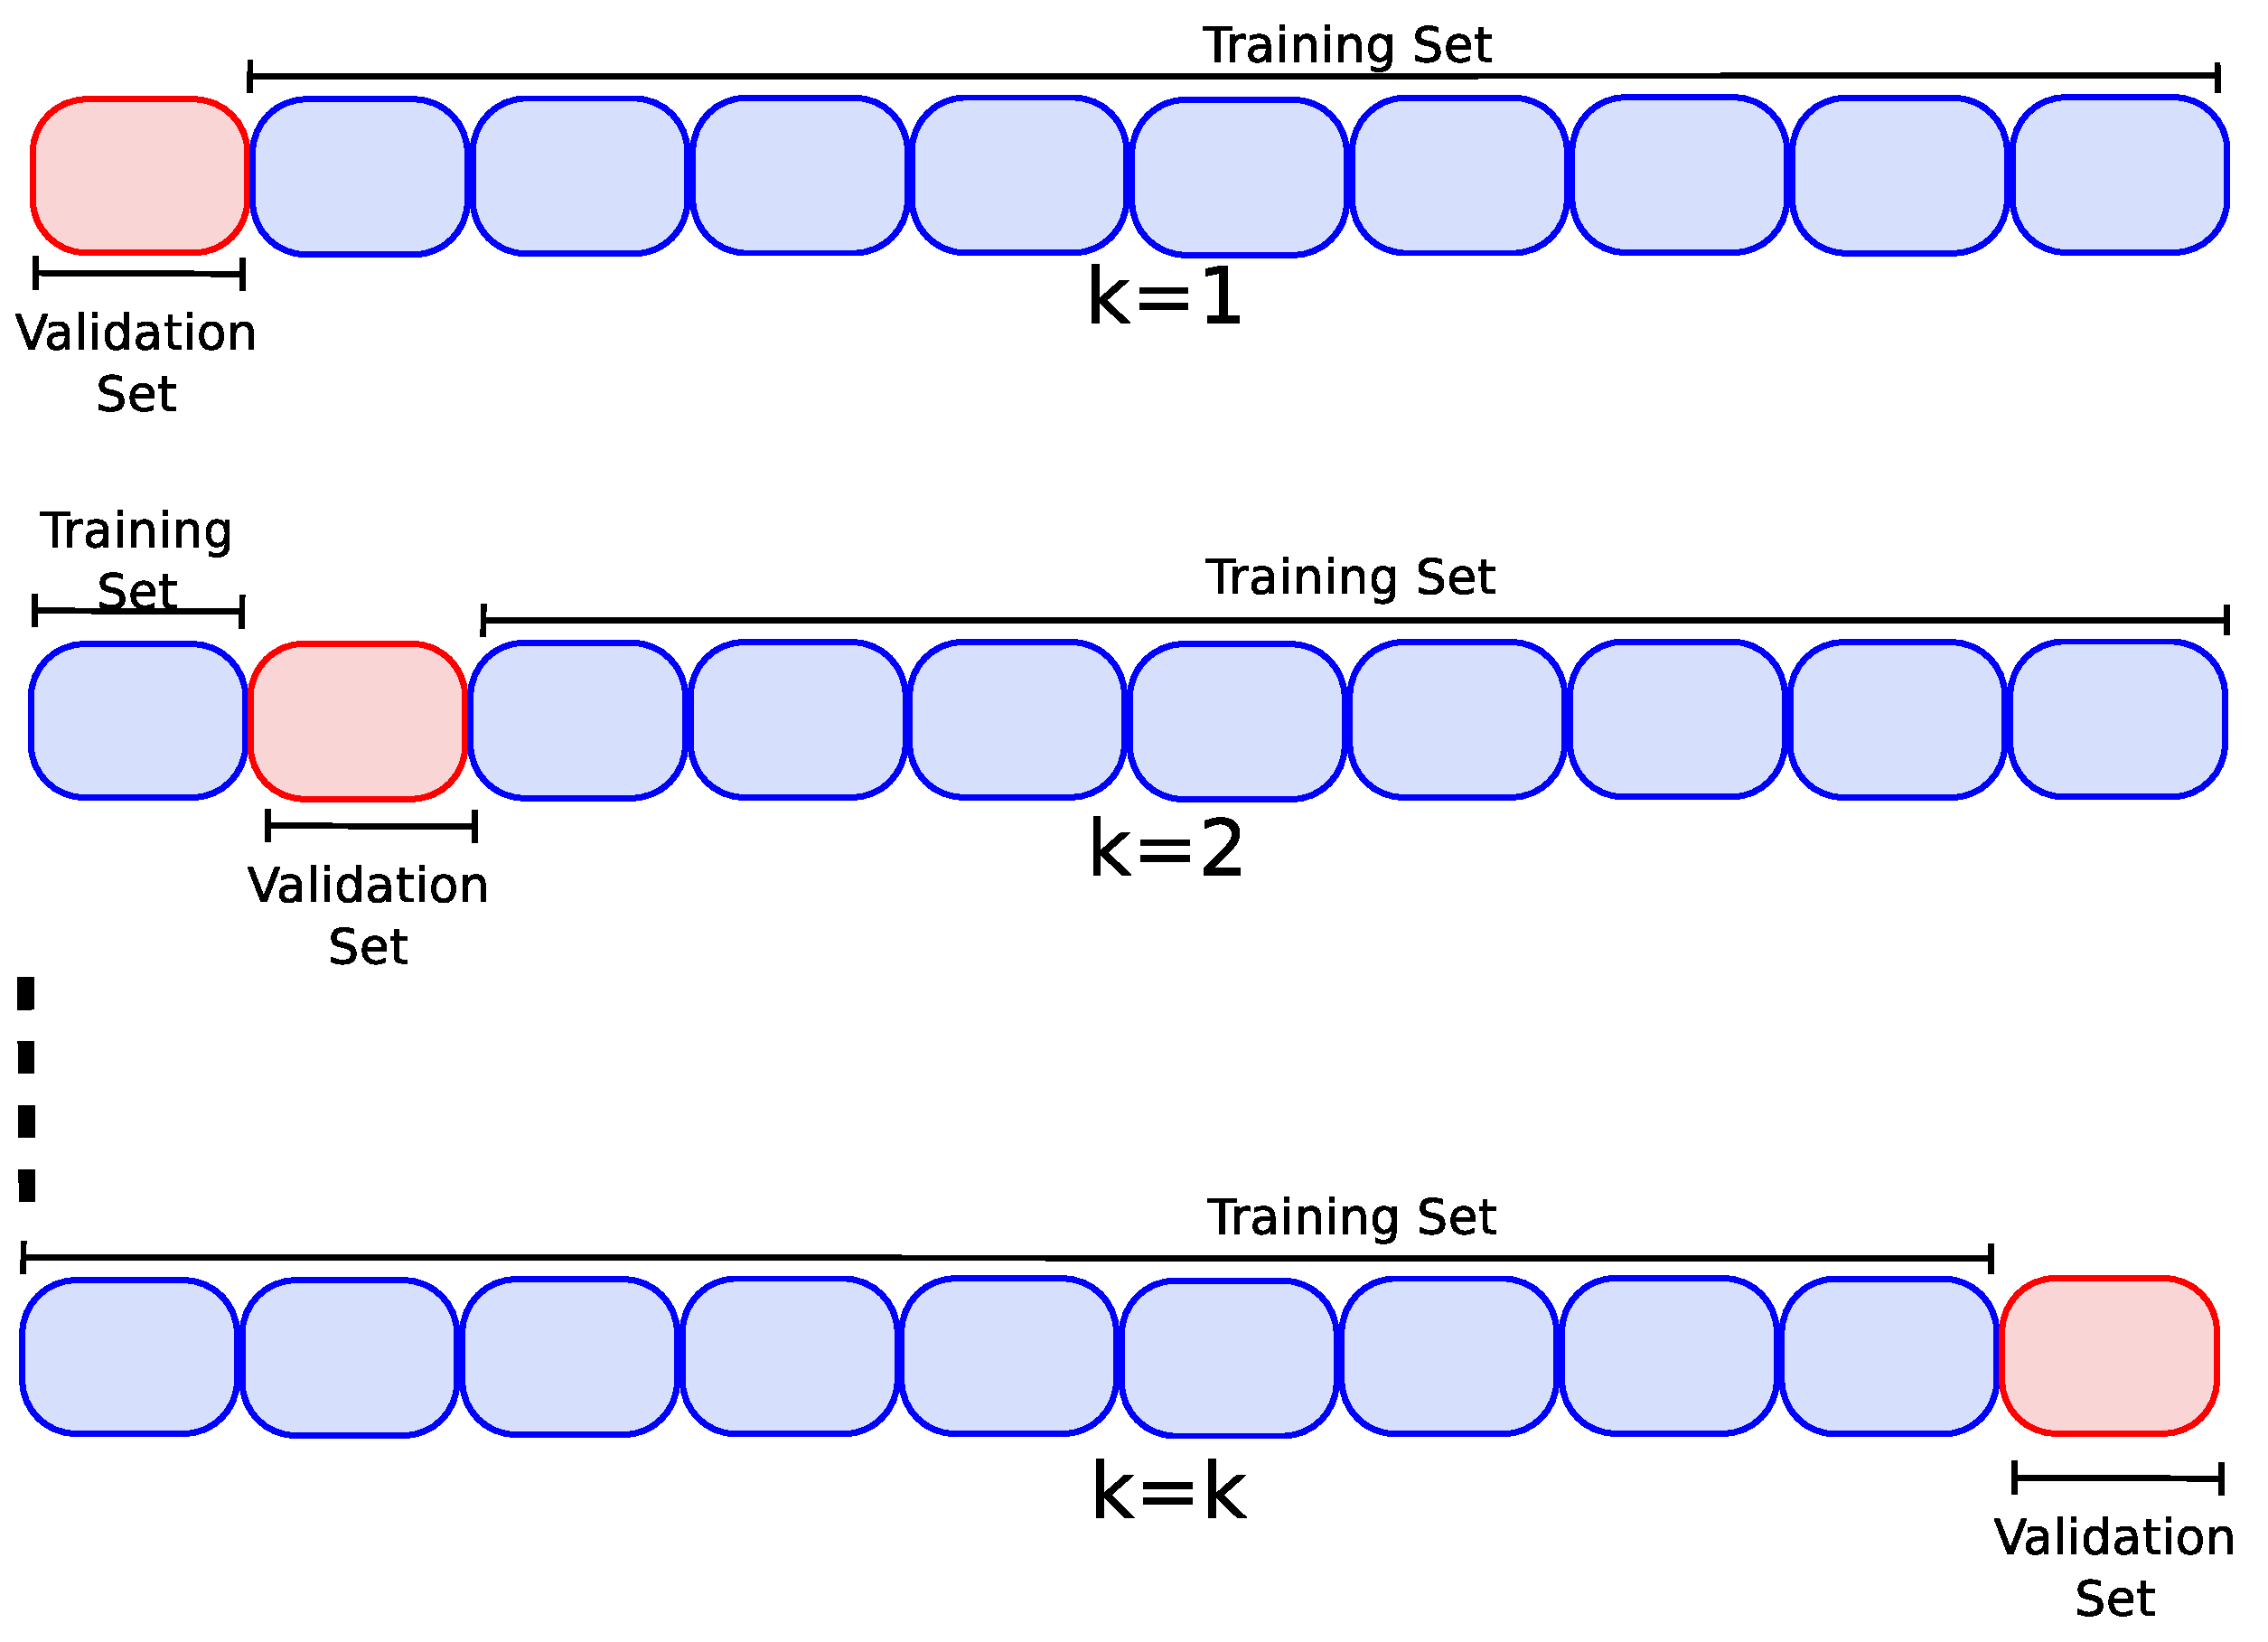
\includegraphics[width=0.75\textwidth]{figures/kfold}
\caption[$k-$fold cross-validation]{Schematic representation of $k$-fold cross-validation technique showing the division of training data into training and validation set. The figure here shows the case when $k$=10.}\label{Fig:kfold}
\end{figure}

On the other hand, if the number of $k$ is large, the bias of the estimator will be significantly low. With large value of $k$, the bias is likely to converge to the true error (generalization error) on the future unseen data. On the contrary, the computational time is greatly increased as the number of iterations increases. For example, in simple $10$-fold cross-validation the learning algorithm is repeated 10 times with $9/10$ of the total data. Additionally, variance of the true error estimate will be significantly larger. In most of the cases, the choice of $k$ depends on the size of dataset. If the size of dataset is larger, smaller number of $k$ is a better option while for smaller datasets larger number of $k$ will be a better option.

The optimal number of $k$ for $k$-fold cross-validation highly researched area but still an open problem.  Although there are some empirical~\cite{Kohavi95astudy} and mathematical results~\cite{witten} suggesting the optimal value of $k$, the choice depends on the rule of thumb. Comprehensive studies and experiments on datasets of different sizes have shown that ten is the optimal number of $k$ to get the accurate error~\cite{witten}. In cross-validation data is randomly divided into $k$ different sets. Hence, different runs of cross-validation with the same learning algorithm on the same data can produce different results. In order to mitigate this problem, different runs (often 10) of the cross-validation procedure is suggested which involves running the learning algorithm 100 times with 9/10 of the total data each time. One $10$-fold cross-validation can be seen as a ``standard'' measure of the performance whereas ten tenfold cross-validations would be a ``precise'' measure of performance~\cite{kayphdthesis}. Furthermore, similar to the problem in hold-out method, cross-validation is also susceptible to ``unfortunate split''. Thus while partitioning the data into subsets, care should be taken to include different unique samples of data in all rows to each of the subset. The idea of `stratification' have been suggested as the solution to the problem of unfortunate split thus ensuring that each class is properly represented in both training and the validation sets. It is important to note that different classes are only approximately represented in the proportion present in the training set.

\section{DNA Copy Number Aberrations Data}
\label{s:copynumberamp}
Humans, being a diploid organism, have two homologous copies of each chromosome usually, one inherited from the father and the other from the mother. During the complex process of cell division, some abnormalities can occur in the cells and copy number changes from two~\cite{aberrations}.  Deletion, often referred to as loss, is the case when the copy number is less than two. Duplication, often referred to as gains, is the case when the copy number is more than two. Amplification is a form of chromosomal aberration when the copy number of the chromosome increases more than 5. Amplification is different from duplication because duplication exactly doubles the copy number. For instance, in human the normal copy number is two, so duplication increases the copy number to 4. Higher level amplifications have been known increases the copy number more than hundred fold. Generally, the amplification is developmentally regulated and amplified copies are lost from the cell. However, amplification in many cases manifests itself in larger number throughout the genome~\cite{aberrations}. DNA amplifications are essentially the hallmarks of cancer. Studies have also shown that copy number amplification results in resistance to certain drugs~\cite{aberrations}. 

CGH (Comparative Genomic Hybridization)~\cite{cgh} is one of the molecular techniques to survey the DNA copy number variation across the whole genome. Differentially labeled test and reference genomic DNA are cohybridized to normal metaphase chromosomes. Fluorescence ratios along the length of the chromosome provide a cytogenetic representation of DNA copy number variation. However, one major drawback of CGH is the resolution. The mapping resolution is only 20Mbp (million base pairs) which is also the average size of the aberrated region. Furthermore, mapping resolution for deletion is 2Mbp. To overcome the problem of CGH, a new microarray technology called aCGH (Array Comparative Genomic Hybridization)~\cite{acgh} has been developed. aCGH provides higher resolution than CGH. Fluorescence ratios at arrayed DNA elements provide a locus by locus measure of the copy number changes. aCGH was initially used to characterize variation in gene expression using cDNA. Using the CGH methods, the chromosome is subbanded to 400 regions, also known as cytogenetic bands. Using different staining techniques, the cytogenetic bands can be visualized and the resolution of the cytogenetic band can be increased to over 800 resolution.

\section[Review of Literature on Copy Number Analysis]{Review of Literature}
\label{s:mmbd}
The problem of analysis of 0-1 data is a very old problem and has been considered extensively in statistics and machine learning. The mixture model is also a well-studied solution. Recently, mixture models have been a subject of major research. For detailed review regarding mixture models and its applications, the reader is referenced to~\cite{mclachlanfmm, mixmodelsreview} and the references therein. On the other hand~\cite{thatreviewarticle} reviews different machine learning methods applied to cancer research. In spite of the great boom of mixture models in the last few decades, comparatively very few instances of research are based on the mixture of multivariate Bernoulli distributions. Nonetheless, the mixture of Bernoulli distribution is found to be suitable in the analysis of the 0-1 data. Thus, this section briefly reviews the research and applications pertaining to the mixture of multivariate Bernoulli distributions with a special focus on cancer genetics. 

The mixture of Bernoulli distributions has found significant application areas when the data is in 0-1 form. For example, in~\cite{binaryimages}, Bernoulli mixture model trained using EM algorithm is used to classify binary images with effective results. In the case of binary image, multiple mixture captures the pixel correlations. Each pixel is assumed to be governed by its associated Bernoulli parameter. One particular application area in which the use of FMM of Bernoulli distributions has excelled is natural language processing. In~\cite{textclassification}, FMM of Bernoulli distributions is used in text classification. The text classification is used to improve the language modelling for machine translation. The text classification is used as an extension to näive Bayes by modelling the class conditional dependence spreading it over different mixture components. In~\cite{textmining}, FMM of Bernoulli distributions has been used in classification. Additionally, the Bernoulli mixture models are used for feature selection and feature extraction including dimensionality reduction from the input data. The combination of the methods implemented in two datasets of varying domains: text mining and hand writing recognition, produces considerable increase in the classification accuracy. Furthermore, the dimensionality reduction of 99.9\% is achieved on the sparse 0-1 data. An interesting and early application of Bernoulli mixture models for statistical modelling of teaching styles is explained in~\cite{Aitkin1981}. The authors compiled a 38 dimensional 0-1 data set of 1258 samples from a questionnaire consisting of 28 items. The mixture modelling technique was tested on 2 to 22 clusters and 12 clusters was selected as it produced the overall maximum. With this statistical modelling techniques, the authors were able to distinguish  different teaching styles.

\subsection{Mixture Models in Copy Number Analysis}
\label{ss:mmcna}
DNA copy number analysis was started in~\cite{pollackgenome} where the authors mainly focused on determining the copy number of the cytogenetic band. Similar works performed are reviewed in~\cite{oldage} to determine the copy number. However, in~\cite{pollackgenome} and~\cite{oldage} the authors did not establish a relation between the copy number and their clinical significance.  In the recent past, DNA copy number amplification data collected with bibliomics survey from 838 journal articles published from 1992 to 2002 was analyzed in~\cite{Myllykangas20067324}. In the work, amplification patterns were determined for 73 different neoplasms and the neoplasms were clustered according to amplification profiles thus identifying the amplification hotspots using independent component analysis. The profiling revealed that human neoplasms formed clusters based on the amplification frequency of the cancer. Continuing the studies in DNA copy number amplification, authors in~\cite{Myllykangas200815} classified the human cancers based on  copy number amplification using probabilistic modelling. Furthermore, the authors extracted the ranges of the amplification in the chromosome and expressed it according to the cytogentic nomenclature. In~\cite{Tikka2007972} and~\cite{Holl20071}, the authors modeled the DNA copy number amplification using a mixture of multivariate Bernoulli Distributions. The classification of 73 different neoplasms in~\cite{Myllykangas20067324} were extended to 95 different neoplasm types. Furthermore, in~\cite{Rancoita2009}, the authors have proposed the enhancement to Bayesian Piecewise Constant Regression(BPCR) called mBPCR changing the segment number estimator and boundary estimator to enhance the fitting procedure. The proposed mBPCR was more accurate in the determination of true breakpoints of amplification. The more recent studies~\cite{Dhaene2010262} and~\cite{Despierre2010358} have mainly focused in cancer specific analysis of DNA copy number. Although the mixture models were used in~\cite{Tikka2007972} and~\cite{Holl20071}, they have studied only chromosome 1 data in resolution 400. Chromosome 1 being the largest chromosome, there is significant amount of amplifications~\cite{Myllykangas20067324}. However, single chromosome band and the specific gene responsible for cancer has not been identified. Hence, in this thesis, study was performed on all chromosomes including chromosome 1. Chromosomewise analysis can reveal interesting facts about amplification of specific chromosomes and guarantees efficient computation \& ease of analysis. Furthermore, there are several sources of multilevel biological data that comes in multiple resolutions as shown in Figure~\ref{Fig:probmultires} but there seems to be a significant gap in research to study multiple resolution of the data as authors in~\cite{Myllykangas20067324} and in relevant work did not consider the data in multiple resolution. Algorithms and methods that meet the demands such multiresolution data could possess very high clinical significance. Thus, this thesis devises methods able to work with multiple resolutions of genome.




